\chapter{Results}
Here we list the evaluation scores, and further guides we use for planning our next steps, available at the time of writing.

\section{Fully Convolutional Network}
Our overall impression with convolutional networks is that, they are slowly training, even high capacity networks are unable to achieve satisfactory score on training set~\ref{fig:convnet-overall}. For this reason, we aimed first to use an architecture, that is capable to over-fit on the train data, so we could fine-tune the training by enforcing the regularization settings.
\paragraph{MLP problem.}
A strange result is that by adding MLP block before the classifier, the performance was drastically reduced, and soon the training collapsed.
The models were biased towards only choosing a single class.
Excellent example for this behavior can be seen on Figure \ref{fig:convnet-bad}, where models with MLP built in oscillate around the same performance throughout an \textit{epoch}. (epoch: a set of training steps which includes every entry from the training set.)
We can also check out the confusion matrix of these models
on Figure \ref{fig:bad-conf-op}, also the histogram of the model parameters reveals, that the network is strongly biased towards choosing one specific class independently from its input in Figure \ref{fig:bad-hist}.

\begin{figure}[h]
  \centering
  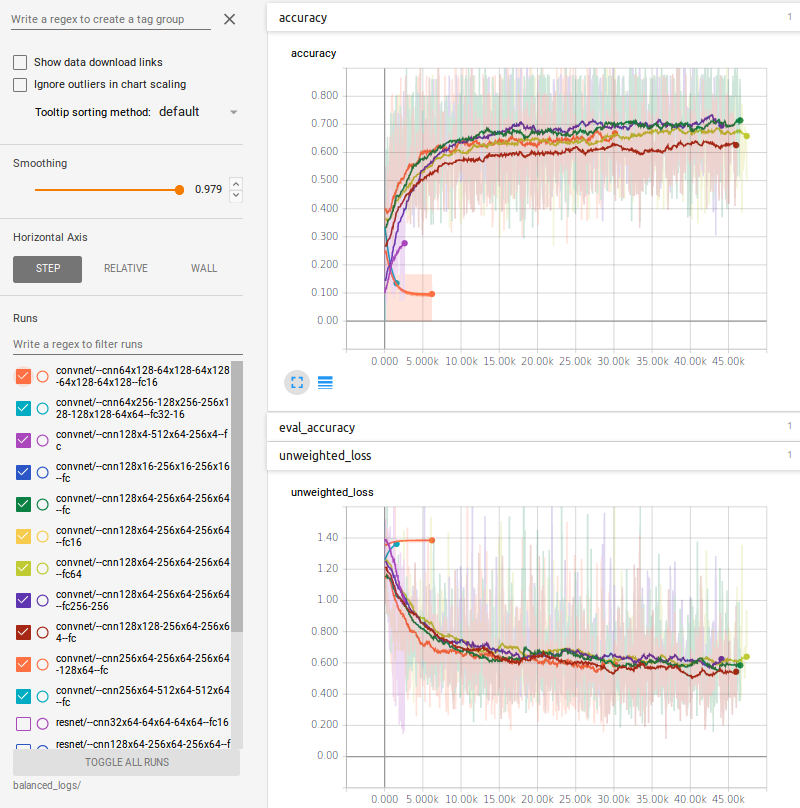
\includegraphics[width=\textwidth]{convnet-overall}\label{fig:convnet-overall}
  \caption{Overall performance of the FCN approaches plotted in TensorBoard. Top: Accuracy derived from the confusion operator. Bottom: Unweighted loss during training}
\end{figure}

\section{Residual Network}
Our next choice were deep residual networks.
With this model, we could achieve better training and evaluation scores.
The exclusion of the MLP block had to be made when using ResNets also, because the same behavior occurred when we applied hidden layers between feature extractors and the classifier layer.

\begin{figure}[h]
  \centering
  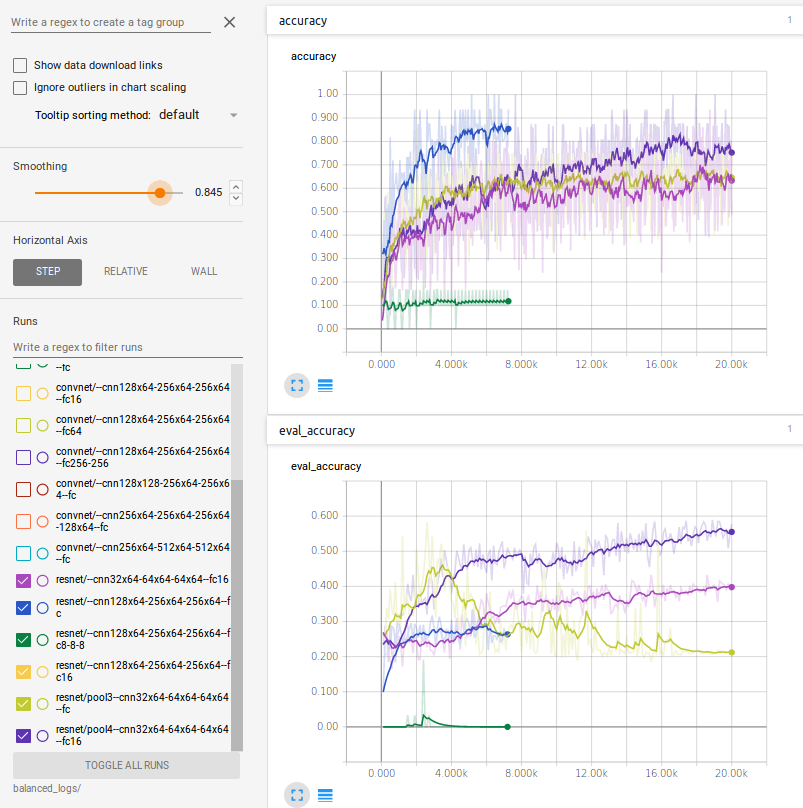
\includegraphics[width=\textwidth]{resnet-overall}\label{fig:resnet-overall}
  \caption{Overall performance of the ResNet approaches plotted in TensorBoard. Top: Accuracy on the training set. Middle: Accuracy on the evaluation set. Bottom: Unweighted loss during training}
\end{figure}
